%!TEX program = xelatex
\documentclass[10pt, compress]{beamer}
\usetheme[titleprogressbar]{m}

\usepackage{booktabs}
\usepackage[scale=2]{ccicons}
\usepackage{minted}
\usepackage{listings}
\usepackage{color}
\usepackage{hyperref}

\usepgfplotslibrary{dateplot}

\usemintedstyle{trac}

\title{\LARGE Ferramentas para análise de séries temporais}
\subtitle{Implementações otimizadas em R}
\author{Aluna: Eduarda Tatiane Caetano Chagas\\Orientador: Alejandro Cesar Frery Orgambide}
\institute{LaCCAN – Laboratório de análise e computação científica}

\begin{document}

\maketitle


\begin{frame}[fragile]
\frametitle{Objetivos do trabalho}
\begin{sloppypar}
\textit{\textbf{\Large "Implementar funções de análise de séries temporais utilizando descritores de Teoria da Informação; implementar uma interface para a aplicação
dessas funções; validar a interface e as funções com usuários finais."}}
\end{sloppypar}
\end{frame}

\begin{frame}[fragile]
\frametitle{Objetivos do trabalho}
\begin{sloppypar}
\textit{\textbf{\Large "\colorbox{gray}{Implementar funções de análise de séries} \colorbox{gray}{temporais utilizando descritores de Teoria} \colorbox{gray}{da Informação}; implementar uma interface para a aplicação
dessas funções; validar a interface e as funções com usuários finais."}}
\end{sloppypar}
\end{frame}

\begin{frame}[fragile]
\frametitle{Séries temporais}
\begin{sloppypar}
\textit{\textbf{\Large "Séries temporais são conjunto de dados obtidos
a partir de um processo observacional ao longo de um determinado período de tempo, não necessariamente dividido em espaços iguais, sendo caracterizadas pela dependência serial existente entre as observações."}}
\end{sloppypar}
\end{frame}

\begin{frame}[fragile]
\frametitle{Séries temporais}
\begin{sloppypar}
\textit{\textbf{\Large "Séries temporais são \colorbox{gray}{conjunto de dados} obtidos
a partir de um processo observacional ao longo de um determinado período de tempo, não necessariamente dividido em espaços iguais, sendo caracterizadas pela dependência serial existente entre as observações."}}
\end{sloppypar}
\end{frame}

\begin{frame}[fragile]
\frametitle{Séries temporais}
\begin{sloppypar}
\textit{\textbf{\Large "Séries temporais são \colorbox{gray}{conjunto de dados} obtidos
a partir de um processo observacional ao longo de um determinado período de tempo, não necessariamente dividido em espaços iguais, sendo caracterizadas pela \colorbox{gray}{dependência serial} existente entre as observações."}}
\end{sloppypar}
\end{frame}

\begin{frame}[fragile]
\frametitle{Áreas de atuação}
\begin{figure}
  \centering
   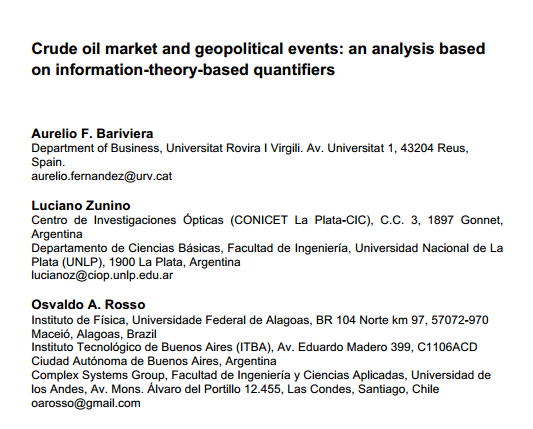
\includegraphics[width=10cm,height=7cm]{CrudeOil.png}
\end{figure}
\end{frame}

\begin{frame}[fragile]
\frametitle{Áreas de atuação}
\begin{figure}
  \centering
   
\includegraphics[width=10cm,height=7cm]{StockMarket.png}
\end{figure}
\end{frame}

\begin{frame}[fragile]
\frametitle{Áreas de atuação}

\begin{figure}
  \centering
   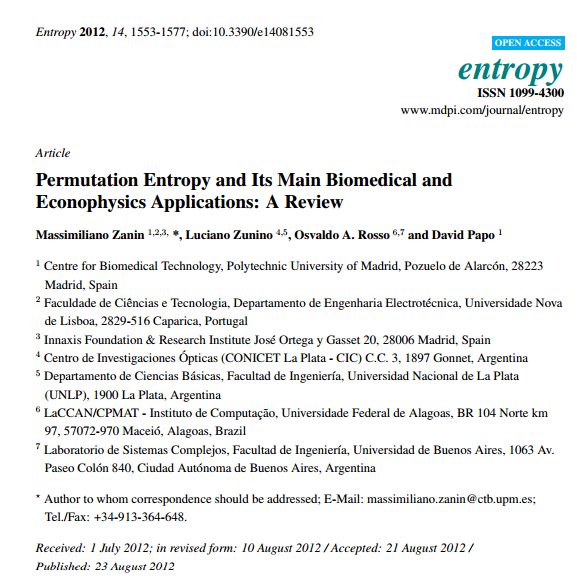
\includegraphics[width=8cm,height=6cm]{Biomedical.png}
\end{figure}
\end{frame}

\begin{frame}[fragile]
\frametitle{Ferramentas presentes}

\begin{figure}
  \centering
   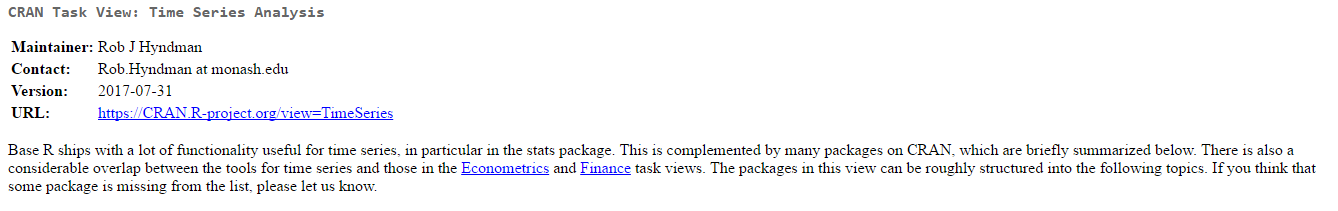
\includegraphics[width=11cm,height=3cm]{CRAN.png}
\end{figure}
\end{frame}

\begin{frame}[fragile]
\frametitle{Ferramentas presentes}

\begin{figure}
  \centering
   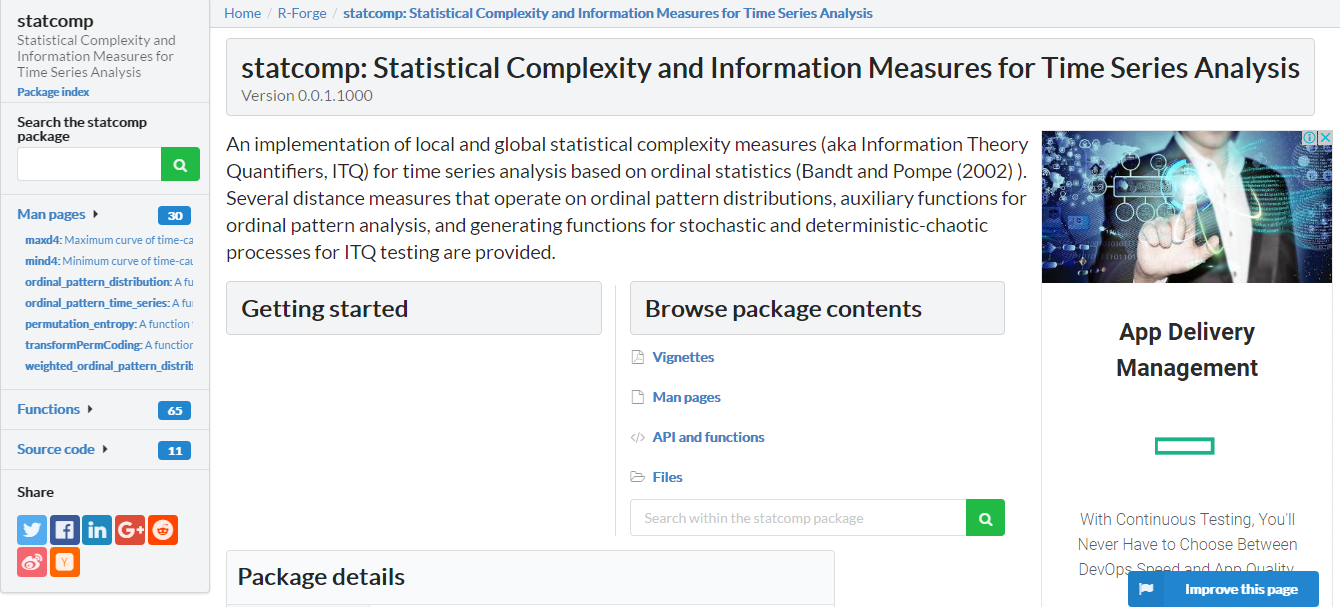
\includegraphics[width=10cm,height=7cm]{statcomp.png}
\end{figure}
\end{frame}

\begin{frame}[fragile]
\frametitle{Objetivo}
 
\textbf{\Large Principais necessidades dos pesquisadores:}\\

-\textit{Ferramenta gráfica amigável;}

-\textit{Funcionalidades
rápidas, eficientes e numericamente confiáveis;} 

-\textit{Portabilidade para diversos
sistemas operacionais e arquiteturas de hardware;}

-\textit{uso de ferramentas FLOSS.} 

\end{frame}

\begin{frame}[fragile]
\frametitle{Metodologia}

\begin{figure}
  \centering
   
\includegraphics[width=10cm,height=5cm]{ferramentas.png}
\end{figure}

\end{frame}


\begin{frame}[fragile]
\frametitle{Metodologia}
 
\textbf{\Large Etapas do processo de análise}\\

\textbf{Simbolização}

-\textit{Processo de simbolização de Bandt e Pompe}\\

\textbf{Extração de informações}

-\textit{Entropias} 

-\textit{Distâncias estocásticas}

-\textit{Complexidade estatística} 

\end{frame}

\begin{frame}[fragile]
\frametitle{Simbolização de Bandt e Pompe}

\begin{figure}
  \centering
   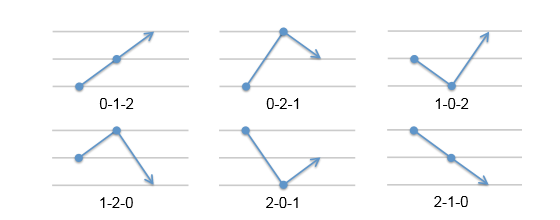
\includegraphics[width=10cm,height=6cm]{p.png}
\end{figure}
\end{frame}


\begin{frame}[fragile]
\frametitle{Histograma}

\begin{figure}
  \centering
   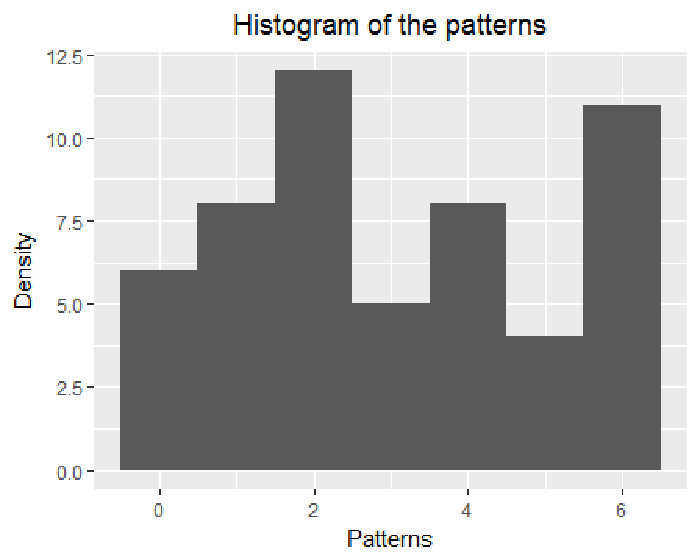
\includegraphics[width=8cm,height=6cm]{Rplot02.pdf}
\end{figure}
\end{frame}

\begin{frame}[fragile]
\frametitle{Entropia}

- Corresponde à medida quantitativa  de incerteza  de uma estrutura descrita por uma distribuição de probabilidade.

\end{frame}

\begin{frame}[fragile]
\frametitle{Entropia de Shannon}

- Seja, assim, $h=(h_1,\dots,h_{N!})$ o histograma de proporções dos $N!$ padrões observados a partir da série temporal $x$.

- Calculamos a entropia de Shannon:

\begin{equation}
 H(h) = \sum_{i=1}^{N!} (-\log h_i) h_i ,
\label{eq:Entropia}
\end{equation}

\end{frame}

\begin{frame}[fragile]
\frametitle{Entropia de Shannon}
 \begin{lstlisting}
H <- function(probability){
  h <- probability * log(probability)
  h[is.nan(h)] <- 0
  return (-sum(h))
}

HNormalized <- function(probability){
  return(H(probability)/log(length(probability)))
}
\end{lstlisting}
\end{frame}


\begin{frame}[fragile]
\frametitle{Entropia de Tsallis}
 \begin{lstlisting}
tsallisEntropy <- function(probability,q,option=0){  
  entropy = sum(probability^q)
  entropy = (1-entropy)*(1/(q-1))
  if(option){
    return (entropy)
  }
  else{
    ent_max=(1-(length(probability)^(1 - q)))/(q-1)
    return( entropy/ent_max)
  }
}
\end{lstlisting}
\end{frame}

\begin{frame}[fragile]
\frametitle{Entropia de Renyi}
 \begin{lstlisting}
renyiEntropy <- function(probability,q,option=0){
  probability = distribution(initial,end)  
  entropy = sum(probability^q)
  entropy = log(entropy)
  entropy = entropy * (1/(1 - q))
  if(option){
    return (entropy)
  }
  else{
    return ( entropy/log(length(probability)))
  }
}
\end{lstlisting}
\end{frame}
 
\begin{frame}[fragile]
\frametitle{ Distância estocástica}

- Mensurando a similaridade entre duas séries temporais, tal medida é calculada através da análise de suas respectivas distribuições de probabilidades.

\end{frame}

\begin{frame}[fragile]
\frametitle{ Distância estocástica}

- Calculamos logo a distância de Jensen-Shannoon à distribuição uniforme $ u=(1/N!,\dots,1/N!)$.

\begin{equation}
D( h, u) = \sum_{i=1}^{N!} \Big(h_i \log\frac{h_i}{u_i} +
u_i \log\frac{u_i}{p_i}
\Big),
\end{equation}

em que $u_i=1/N!$.
\end{frame}

\begin{frame}[fragile]
\frametitle{Distâncias estocásticas}
 \begin{lstlisting}
euclidian_distance<-function(probability){
  c = rep(1/length(probability),length(probability))
  distance = sum((probability-c)^2)
  return(sqrt(distance))
}
euclidian_quadratica_distance<-function(probability){
  c = rep(1/length(probability),length(probability))
  distance = sum((probability-c)^2)
  return(distance)
}
manhattan_distance<-function(probability){
  c = rep(1/length(probability),length(probability))
  distance = sum(abs(probability-c))
  return(distance)
}
\end{lstlisting}
\end{frame}


\begin{frame}[fragile]
\frametitle{Distâncias estocásticas}
 \begin{lstlisting}
kullback_leibler_divergence<-function(probability){
  c = rep(1/length(probability),length(probability))
  distance <- probability * log(probability/c)
  distance[is.nan(distance)] <- 0
  return(sum(distance))
}
\end{lstlisting}
\end{frame}

\begin{frame}[fragile]
\frametitle{Distâncias estocásticas}
 \begin{lstlisting}
hellinger_Distance<-function(probability){
  c = rep(1/length(probability),length(probability))
  distance = sum((sqrt(probability)-sqrt(c))^2)*0.5
  return(sqrt(distance))
}

jensenDivergence<-function(p){
  q = rep(1/length(p),length(p))
  s_p = shannonEntropy(p)
  s_q = shannonEntropy(q)
  s_pq = shannonEntropy((p+q)/2)
  divergence = sum( s_pq - (s_p/2) - (s_q/2))
  return(divergence)
}
\end{lstlisting}
\end{frame}

\begin{frame}[fragile]
\frametitle{Distâncias estocásticas}
 \begin{lstlisting}
wootters_distance<-function(probability,q){
  c = rep(1/length(probability),length(probability))
  dis = sum(sqrt(probability*c))
  dis = acos(dis)
  return(dis)
}
chebyshev_distance<-function(probability){
  c = rep(1/length(probability),length(probability))
  L = abs(probability - c)
  return(max(L))
}
\end{lstlisting}
\end{frame}

 
\begin{frame}[fragile]
\frametitle{Complexidade estatística}

- Procura encontrar estruturas de interação
de dependência entre os elementos de uma dada série.

\end{frame}
 
\begin{frame}[fragile]
\frametitle{Complexidade estatística}

- Calculamos o segundo descritor da nossa série temporal: a sua Complexidade Estatística:

\begin{equation}
C( h, u) = H( h) D( h,  u).
\end{equation}

\end{frame}

\begin{frame}[fragile]
\frametitle{ Plano Complexidade-Entropia}

- Cada série temporal pode então ser descrita por um ponto $(H( h), C( h,  u))$.
O conjunto de todos os pares $(H( h), C( h,  u))$ para qualquer série temporal descrita por padrões de comprimento $N$ jaz em um subconjunto compacto $ R^2$: o plano Entropia-Complexidade.

\end{frame}

\begin{frame}[fragile]
\frametitle{ Plano Complexidade-Entropia}

\begin{figure}
  \centering
   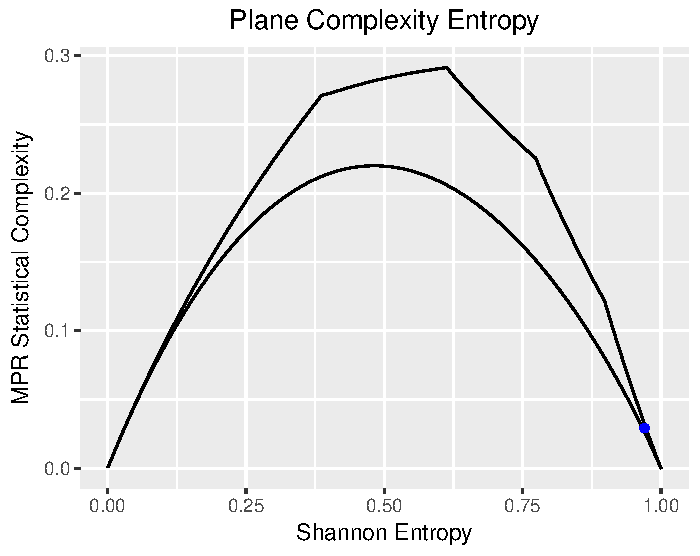
\includegraphics[width=8cm,height=6cm]{Rplot3.pdf}
\end{figure}
\end{frame}

\begin{frame}[fragile]
\frametitle{ Série Temporal}

\begin{figure}
  \centering
   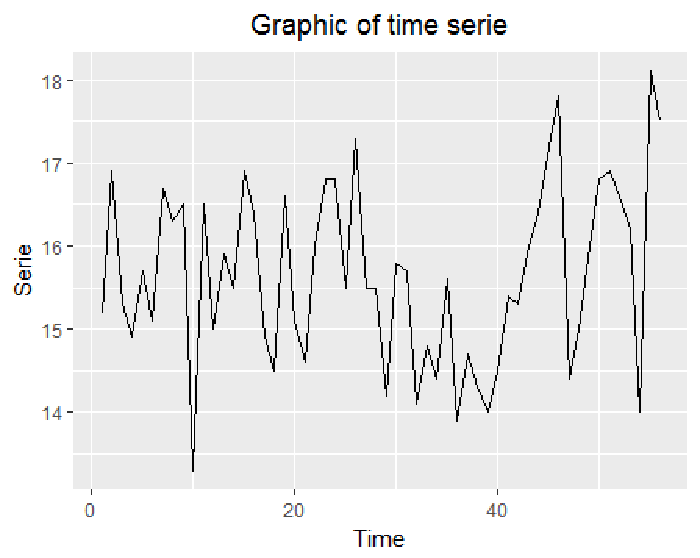
\includegraphics[width=8cm,height=6cm]{Rplot.pdf}
\end{figure}
\end{frame}

\begin{frame}[fragile]
\frametitle{ Série Temporal e os padrões}

\begin{figure}
  \centering
   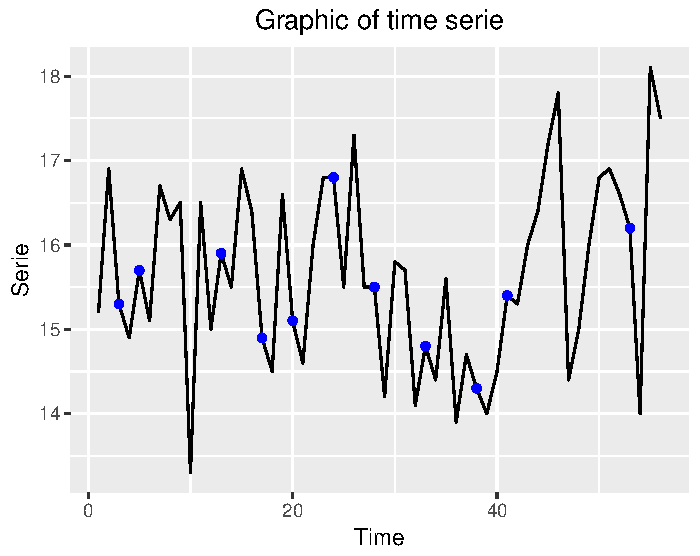
\includegraphics[width=8cm,height=6cm]{Rplot04.pdf}
\end{figure}
\end{frame}

\begin{frame}[fragile]
\frametitle{Mineração de dados}

- Possuem como característica reduzir substâncialmente o tamanho dos dados, porém mantendo intactas suas principais características.
\end{frame}

\begin{frame}[fragile]
\frametitle{Piecewise Aggregate Aproximation}
\begin{figure}
  \centering
   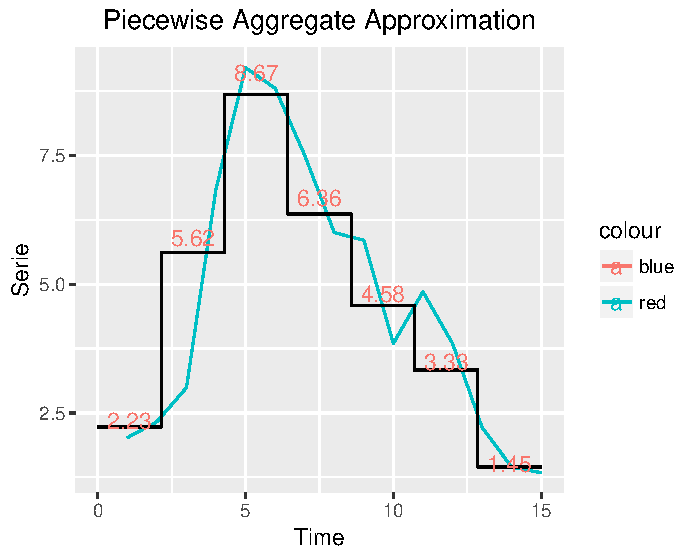
\includegraphics[width=10cm,height=6cm]{PAA.pdf}
\end{figure}
\end{frame}

\begin{frame}[fragile]
\frametitle{Perceptually Important Points}
\begin{figure}
  \centering
   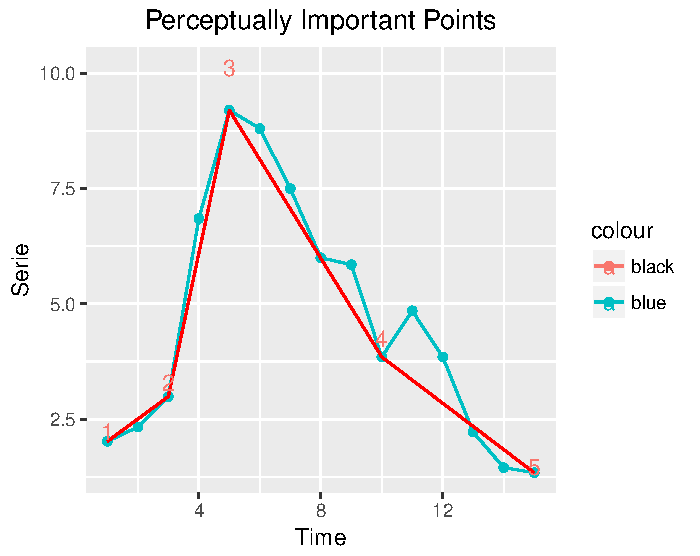
\includegraphics[width=10cm,height=6cm]{PIP.pdf}
\end{figure}
\end{frame}

\begin{frame}[fragile]
\frametitle{Symbolic Aggregate Approximation}
\begin{figure}
  \centering
   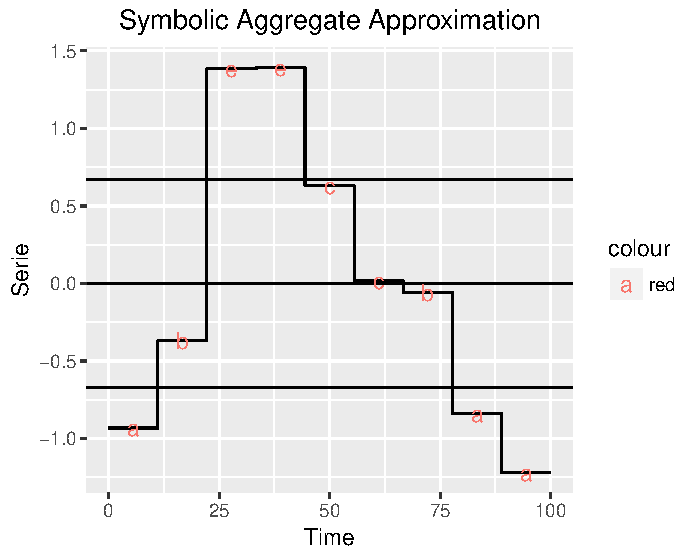
\includegraphics[width=10cm,height=6cm]{SAX.pdf}
\end{figure}
\end{frame}

\begin{frame}[fragile]
\frametitle{Sistema}

- O sistema for projetado e desenvolvido de forma modular, composto pelas seguintes unidades:

\begin{itemize}
\item Módulo de simbolização;
\item Módulo de análise;
\item Modulo de visualização e interação;
\end{itemize} 

\end{frame}

\begin{frame}[fragile]
\frametitle{Sistema}

- Para aumentar a aplicabilidade do sistema, permite-se a tanto a geração de séries quanto a leitura de dados em vários formatos (TXT, CSV ou XLSX), e o usuário a seguir escolhe:

\begin{itemize}
\item Gerar o gráfico da série;
\item Calcular diversos tipos de Entropia;
\item Calcular diversos tipos de Distâncias Estocásticas;
\item Calcular complexidades estatísticas;
\item Gerar o histograma de padrões;
\item Identificar o ponto característico da série no plano Entropia-Complexidade.
\end{itemize}

\end{frame}

\begin{frame}[fragile]
\frametitle{Objetivos do trabalho}
\begin{sloppypar}
\textit{\textbf{\Large "Implementar funções de análise de séries temporais utilizando descritores de Teoria da Informação; \colorbox{gray}{implementar uma interface para a aplicação}
\colorbox{gray}{dessas funções}; validar a interface e as funções com usuários finais."}}
\end{sloppypar}
\end{frame}

\begin{frame}[fragile]
\frametitle{Interface gráfica}
\begin{figure}
  \centering
   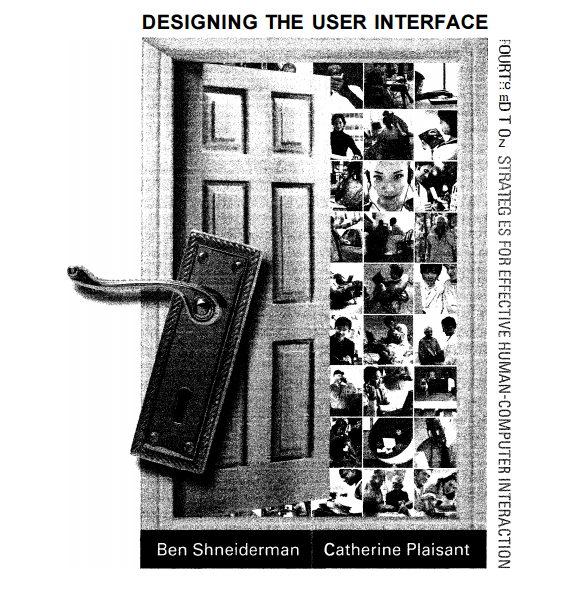
\includegraphics[width=6cm,height=6cm]{interface.png}
\end{figure}
\end{frame}

\begin{frame}[fragile]
\frametitle{Interface gráfica}

-\textbf{ \Large Regras de Ouro de Shneiderman:}

\begin{itemize}
\item Esforce-se pela consistência;
\item Atender a usabilidade universal;
\item Oferecer um feedback informativo;
\item Diálogos que indiquem o fim de uma ação;
\item Evite erros;
\item Permitir a fácil reversão de ações;
\item Suportar o controle do usuário;
\item Reduzir a carga de memória de curta duração.
\end{itemize}
\end{frame}

\begin{frame}[fragile]
\frametitle{Interface gráfica}
\begin{figure}
  \centering
   
\includegraphics[width=10cm,height=6cm]{FInterface.png}
\end{figure}
\end{frame}

\begin{frame}[fragile]
\frametitle{Interface gráfica}
\begin{figure}
  \centering
   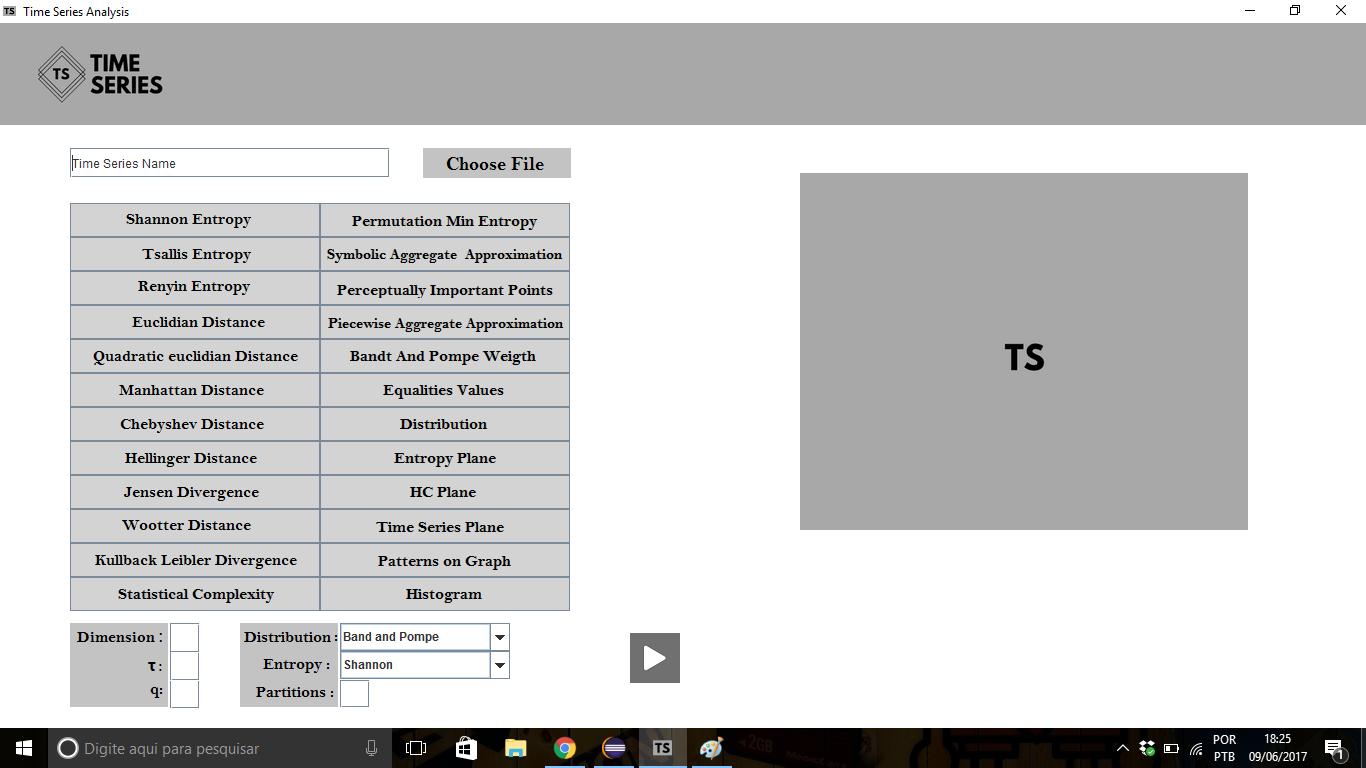
\includegraphics[width=10cm,height=6cm]{tela4.png}
\end{figure}
\end{frame}

\begin{frame}[fragile]
\frametitle{Interface gráfica}
\begin{figure}
  \centering
   
\includegraphics[width=10cm,height=6cm]{rgtk2.png}
\end{figure}
\end{frame}

\begin{frame}[fragile]
\frametitle{Objetivos futuros do trabalho}
\begin{sloppypar}
\textit{\textbf{\Large "Implementar funções de análise de séries temporais utilizando descritores de Teoria da Informação; implementar uma interface para a aplicação dessas funções; \colorbox{gray}{validar a interface e as funções com usuários} \colorbox{gray}{finais}."}}
\end{sloppypar}
\end{frame}

\begin{frame}[fragile]
  \frametitle{Referências}
Referências: 
\begin{itemize}

\item{Characterization of vehicle behavior with Information Theory / Aquino, A. L. L. et al. (2015)}

\item{A Mathematical Theory of Communication / Shannon, C. E. (1948)}

\item{Measures of statistical complexity: Why? / Feldman and Crutcheld (1998)}

\item{Permutation entropy: A natural complexity measure for time series / Bandt and Pompe (2002)}

\end{itemize}
\end{frame}

\plain{Dúvidas?}

\end{document}